\phantomsection
\definecolor{dkgreen}{rgb}{0,0.6,0}
\definecolor{gray}{rgb}{0.5,0.5,0.5}
\definecolor{mauve}{rgb}{0.58,0,0.82}


\lstset{frame=tb,
language=R,
aboveskip=3mm,
belowskip=3mm,
showstringspaces=false,
columns=flexible,
numbers=none,
inputencoding=utf8/latin1,
keywordstyle=\color{blue},
numberstyle=\tiny\color{gray},
commentstyle=\color{dkgreen},
stringstyle=\color{mauve},
breaklines=true,
breakatwhitespace=true,
tabsize=3
}

\chapter{Statistica Descrittiva Bivariata}\label{cap4}

In questo capitolo si sviluppa la statistica descrittiva bivariata, ossia il ramo della statistica che si occupa dei metodi grafici e statistici atti a descrivere le relazioni tra \textit{due} variabili quantitative.

Dopo aver scelto la variabile da porre sulle ascisse (variabile indipendente) \textit{X} e la variabile da porre sulle ordinate (variabile dipendente) \textit{Y}, si disegnano dei punti in corrispondenza delle coppie ($x_i, y_i$). Ciò che si ottiene disegnando tali punti mediante \textit{diagrammi di dispersione} (scatterplot) è una nuvola di punti che evidenzia, se esiste, una qualche \textit{forma di regolarità}, o meglio una qualche \textit{forma di relazione} tra le variabili.

In particolare si analizzeranno le relazioni tra i dati presenti attraverso indici di covarianza campionaria, coefficiente di correlazione campionario e vari grafici. Successivamente si andrà ad osservare la regressione lineare semplice, multipla e non lineare.

\section{Covarianza e correlazione campionaria}\label{cap4.1}

Spesso nelle indagini statistiche si osservano più variabili quantitative per uno stesso gruppo di individui e, in tal caso, è necessario vedere se esiste una correlazione tra le variabili.

\subsection{Covarianza campionaria}\label{cap4.1.1}

Per ottenere una misura quantitativa della correlazione tra le variabili si considera la \textit{covarianza campionaria}.

\noindent \textbf{Definizione:} Assegnato un campione bivariato ($x_1, y_1$), ($x_2, y_2$), ..., ($x_n, y_n$), di una variabile quantitativa bidimensionale (X, Y), siano $\bar x$ e $\bar y$ rispettivamente le medie campionarie di $x_1, x_2, ..., x_n$ e di $y_1, y_2, ..., y_n$. La \textbf{\textit{covarianza campionaria}} tra le due variabili X e Y è così definita:

\[C_{xy} = \frac{1}{n-1} \sum_{i=1}^n (x_i - \bar x)(y_i - \bar y) \quad \quad (n = 2, 3, ...)\]

In R la covarianza campionaria può essere facilmente calcolata con la funzione \textit{cov}

\vspace{5mm}
\noindent \textbf{Covarianza Campionaria delle caratteristiche del dataset}

\vspace{5mm}
\begin{lstlisting}
round(cov(df),digits = 2)
\end{lstlisting}
\vspace{5mm}

\vspace{5mm}
\begin{tabular}{c c c c c}
 & Modo.Cont. & Modo.Salt. & Qualche.Att & Non.Prat.Sport\\
 Modo.Cont. & 41.67 & 13.49 & 16.49 & -71.80\\
 Modo.Salt. & 13.49 & 6.20 & 7.21 & -26.92\\
 Qualche.Att. & 16.49 & 7.21 & 18.04 & -41.82\\
 Non.Prat.Sport & -71.80 & -26.92 & -41.82 & 140.83\\
\end{tabular}
\vspace{5mm}

Osservando i valori della covarianza si può notare come nella maggior parte dei casi i valori sono positivi ($C_{xy} > 0$), ovvero le variabili associate a tali valori sono correlate positivamente. Valori troppo bassi, però, denotano una scarsa correlazione. Nella colonna della caratteristica Non Praticano Sport, alcuni dei valori sono però negativi, simbolo di una correlazione negativa. Possiamo notare come sulla diagonale sono presenti i valori della varianza osservati in precedenza.

\subsection{Correlazione campionaria}\label{cap4.1.2}

Per ottenere una misura quantitativa della correlazione tra le variabili si può anche considerare il coefficiente di correlazione campionario 

\noindent \textbf{Definizione:} Assegnato un valore bivariato ($x_1, y_1$), ($x_2, y_2$), ..., ($x_n, y_n$) di una variabile quantitativa bidimensionale (X,Y) siano $\bar x$ e $s_x$ la media campionaria e la deviazione standard campionaria di $x_1, x_2, ..., x_n$ e siano $\bar y$ e $s_y$  la media campionaria e la deviazione standard campionaria di $y_1, y_2, ..., y_n$. Il \textbf{\textit{coefficiente di correlazione campionario}} tra le due variabili X e Y è così definito:

\[r_{xy} = \frac{C_{xy}}{s_{x} s_{y}}\]

In R il coefficiente di correlazione campionario può essere facilmente calcolato con la funzione \textit{cor()}.

\noindent \textbf{Coefficiente di correlazione delle caratteristiche del dataset}

\vspace{5mm}
\begin{lstlisting}
    round(cor(df), digits = 2)
\end{lstlisting}
\vspace{5mm}

\vspace{5mm}
\begin{tabular}{c c c c c}
 & Modo.Cont. & Modo.Salt. & Qualche.Att & Non.Prat.Sport\\
 Modo.Cont. & 1.00 & 0.84 & 0.60 & -0.94\\
 Modo.Salt. & 0.84 & 1.00 & 0.68 & -0.91\\
 Qualche.Att. & 0.60 & 0.68 & 1.00 & -0.83\\
 Non.Prat.Sport & -0.94 & -0.91 & -0.83 & 1.00\\
\end{tabular}
\vspace{5mm}

In modo analogo alla covarianza campionaria, il coefficiente di correlazione campionario indica la relazione tra i dati del campione, ottenendo anche in questo caso non soltanto correlazioni positive ma anche negative. Si nota che sulla diagonale troviamo il valore 1 poiché una caratteristica è correlata al massimo con se stessa con tutti i punti allineati su una \textbf{linea retta ascendente}, mentre gli altri valori indicano un rapporto di relazione non influenzato dalle unità di misura dei dati. Il coefficiente di correlazione campionario, inoltre, indica che se 0 < $r_{xy}$ < 1 allora i punti $x_i, y_i$ sono posizionati in una nuvola attorno a una linea \textbf{retta interpolante ascendente}, mentre se -1 < $r_{xy}$ < 0 allora i punti $x_i, y_i$ sono posizionati in una nuvola attorno a una linea \textbf{retta interpolante discendente}

\section{Regressione lineare semplice}\label{cap4.2}

Il \textit{modello di regressione lineare} semplice è esprimibile attraverso l'equazione di una retta che riesce a interpolare la nuovola di punti dello scatterplot meglio di tutte le altre possibili rette. Consideriamo l'equazione della retta: 

\[Y = \alpha + \beta X\]

\noindent dove

\begin{itemize}
    \item $\alpha$ è l'intercetta: corrisponde all'ordinata del punto di intersezione della retta interpolante (di regressione) con l'asse delle ordinate.
    \item $\beta$ è il coefficiente angolare: esprime l'inclinazione della retta.
\end{itemize}

In questo paragrafo si andrà ad analizzare la regressione lineare semplice per un sottoinsieme di dati, poiché analizzare tutto il dataset risulterebbe oneroso. Lo studio della regressione lineare semplice verrà effettuato sulla base di due caratteristiche del dataset, ponendo:

\begin{itemize}
    \item \textbf{Variabile indipendente: Modo Continuativo}
    \item \textbf{Variabile dipendente: Qualche Attività}
\end{itemize}

\noindent \textbf{Scatterplot delle due variabili considerate}

Con il seguente codice si va a disegnare lo scatterplot (diagramma di dispersione) delle due variabili.

\begin{figure}[!htbp]
    \centering
    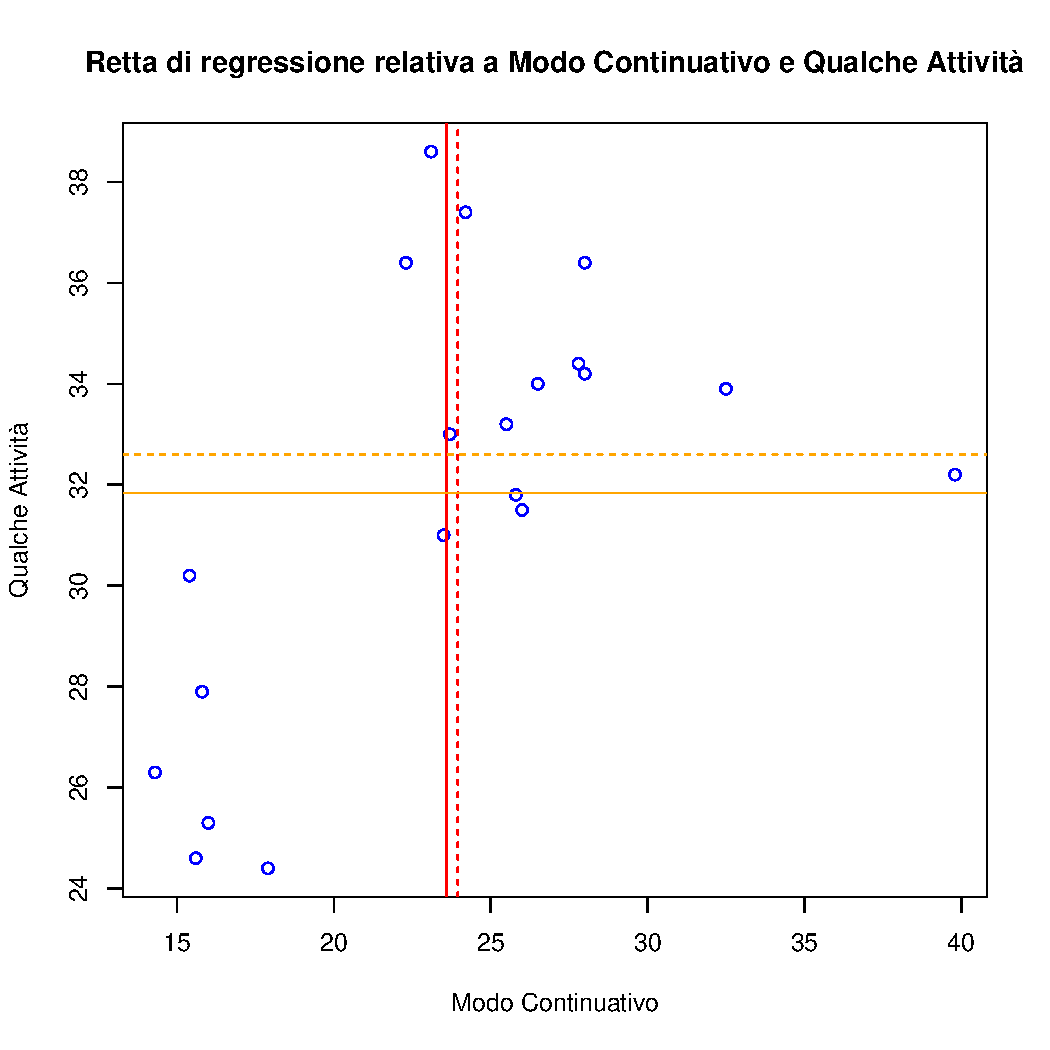
\includegraphics[height=16cm]{ProgettoSAD/capitoli/images/s_desc_biv/scatterplot_variabili.pdf}
\end{figure}

Dal grafico ottenuto si nota che la nuvola di dati sembra posizionarsi intorno a una retta ascendente, inducendo a pensare che esista una correlazione lineare positiva tra entrambe le variabili. Nel grafico sono anche stati evidenziati i valori della media (linea retta) e della mediana (linea tratteggiata) per entrambe le caratteristiche che appaiono rosse per la caratteristica Modo Continuativo e arancioni per la caratteristica Qualche Attività.

\noindent \textbf{Calcolo della retta di regressione}

Al fine di poter disegnare la retta di regressione ($Y = \alpha + \beta X$) che interpola i punti nel grafico si vanno a calcolare i parametri $\alpha$ e $\beta$ di tale retta con il seguente codice, impiegando la funzione \textit{lm(y $\sim$ x)(linear model)}.

\vspace{5mm}
\begin{lstlisting}
  lm_reg <- lm(df$Qualche.Att. ~ df$Modo.Cont.)
  lm_reg

    Call:
    lm(formula = df$Qualche.Att. ~ df$Modo.Cont.)
    
    Coefficients:
      (Intercept)  df$Modo.Cont.  
          22.5033         0.3957    
\end{lstlisting}
\vspace{5mm}
 
Disegnando, attraverso la funzione \textit{abline(lm\_reg)} la retta

\[Y = 22.5033 + 0.3957X\]

sul grafico precedente

\vspace{5mm}
\begin{lstlisting}
  plot(df$Modo.Cont., df$Qualche.Att., main = " Retta di regressione relativa a
  Modo Continuativo e Qualche Attività ",
       xlab = " Modo Continuativo ",
       ylab = " Qualche Attività ", col = " blue ")
  abline(rettaRegressione(df), col = " red ")
\end{lstlisting}
\vspace{5mm}

si ottiene:

\begin{figure}[!htbp]
    \centering
    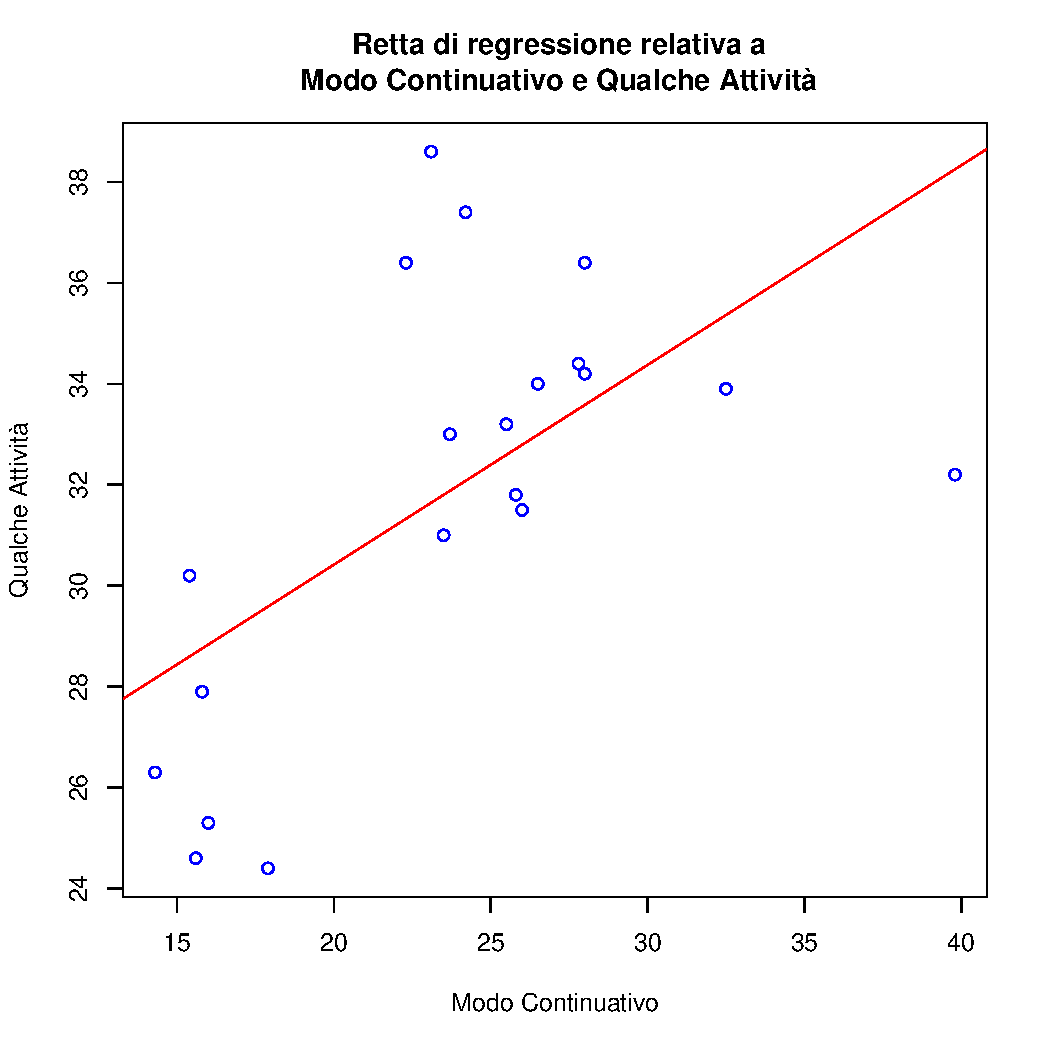
\includegraphics[height=16cm]{ProgettoSAD/capitoli/images/s_desc_biv/retta_regressione.pdf}
\end{figure}

\subsection{Residui}\label{cap4.2.1}

Una volta calcolati i valori dei coefficienti $\alpha$ e $\beta$ e disegnata la retta di regressione che interpola la nuvola dei punti nel corrispondente scatterplot, è possibile osservare quanto questa retta si adatta ai punti che individuano le osservazioni. 

In generale, esisteranno degli scostamenti (\textbf{residui}) tra le ordinate dei punti $y_i$ (\textit{valori osservati)} e i corrispondenti \textit{valori stimati}

\[\hat{y_i} = \alpha + \beta x_i \quad \quad (i = 1, 2, ..., n)\]

ottenuti mediante la retta di regressione. I punti ($x_1, \hat{y_1}$), ($x_2, \hat{y_2}$), ..., ($x_n, \hat{y_n}$) sono posizionati sulla retta di regressione. 

I residui,

\[E_i = y_i - \hat{y_i} = y_i - (\alpha + \beta x_i) \quad \quad (i = 1, 2, ..., n)\]

dunque, mostrano di quanto si discostano i valori osservati dai valori stimati con la retta di regressione. Inoltre, la media campionaria dei residui $E$ è nulla, ossia in media gli scostamenti positivi e negativi si compensano

\noindent \textbf{Valori stimati}

In R per calcolare il vettore dei valori stimati ($\hat{y_1}, \hat{y_2}, ..., \hat{y_n}$) si utilizza la funzione \textit{fitted()}, ottenendo:

\vspace{5mm}
\begin{lstlisting}
    stime <- fitted(lm(df$Modo.Cont. ~ df$Qualche.Att.))
    stime


       1        2        3        4        5 
32.79052 35.36232 31.64310 33.58184 38.25064 
       6        7        8       9       10 
33.50271 32.07833 33.58184 32.98835 31.8805 
      11       12       13       14       15
32.59269 32.71139 31.80137 28.59652 28.16129
      16      17       18       19       20 
29.58567 28.83391 28.75478 28.67565 31.32658 
\end{lstlisting}
\vspace{5mm}

Ad esempio, il primo valore stimato (32.79) è il risultato di $\hat{y_1} = \alpha + \beta x_1 = 22.5033 + 0.3957 * 26$, dove 26 è il dato percentuale del primo elemento del dataset nella \textit{caratteristica indipendente} (Modo Continuativo).

\vspace{5mm}
\noindent \textbf{Residui}
\vspace{5mm}

In R per calcolare il vettore dei residui ($E_1, E_2, ..., E_n$) si utilizza la funzione \textit{resid()}, ottenendo:

\vspace{5mm}
\begin{lstlisting}
    residui <- resid(lm(df$Qualche.Att. ~ df$Modo.Cont.))
    residui


         1          2          3          4          5
-1.2905206 -1.4623152  6.9568954  2.8181580 -6.0506384
         6          7          8          9         10
 0.8972901  5.3216687  0.6181580  1.0116490  1.1194990
        11         12         13         14         15
 0.6073097 -0.9113885 -0.8013688  1.6034829 -1.8612903 
        16         17         18         19         20 
-5.1856689 -3.5339135 -0.8547814 -4.0756492  5.0734240
\end{lstlisting}
\vspace{5mm}

Ad esempio, il primo valore stimato (-1.29) è il risultato di $y_1 - \hat{y_1} = 31.5 - 32.79 $, dove 31.5 è il dato percentuale del primo elemento del dataset nella \textit{caratteristica dipendente} (Qualche Attività), mentre 32.79 è il valore stimato precedentemente.

\vspace{5mm}
\noindent \textbf{Disegno dei Residui}

Il seguente codice disegna i residui, ovvero dei segmenti che congiungono i \textit{valori stimati} (punti sulla retta) e i \textit{valori osservati}.

\vspace{5mm}
\begin{lstlisting}
  plot(df$Modo.Cont., df$Qualche.Att., main = " Retta di regressione relativa
  a Modo Continuativo e Qualche Attività ",
       xlab = " Modo Continuativo ",
       ylab = " Qualche Attività ", col = " blue ")
  abline(rettaRegressione(df), col = " red ")
  segments(df$Modo.Cont., fitted(lm(df$Qualche.Att. ~ df$Modo.Cont.)), 
           df$Modo.Cont., df$Qualche.Att., col = "green ")
\end{lstlisting}
\vspace{5mm}

\vspace{5mm}
\begin{figure}[!htbp]
    \centering
    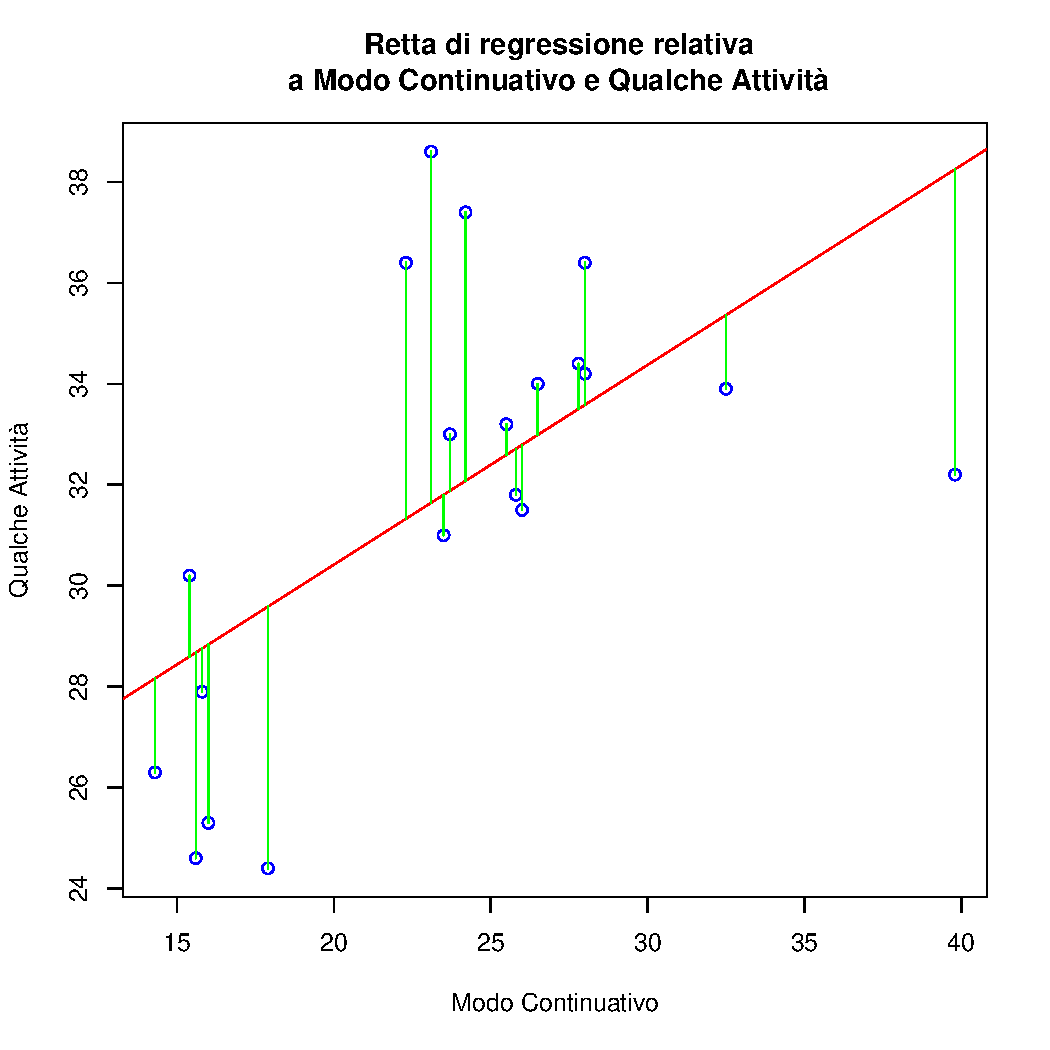
\includegraphics[height=16cm]{ProgettoSAD/capitoli/images/s_desc_biv/disegno_residui.pdf}
\end{figure}
\vspace{5mm}

Attraverso la funzione \textit{segments()} è stato possibile disegnare dei segmenti in modo tale da poter osservare gli scostamenti tra i valori stimati e i valori osservati.

\vspace{5mm}
\noindent \textbf{Diagramma dei residui}

Un esame più accurato del modo con cui la retta di regressione interpola i dati e di come i residui si dispongano intorno alla retta interpolante influenzandone la posizione può essere ottenuto attraverso il \textit{diagramma dei residui}, che è un grafico in cui i \textit{valori dei residui} sono posti sull'asse delle ordinate e quelli della \textit{variabile indipendente} sull'asse delle ascisse. Di seguito il codice per costruire il diagramma dei residui con il relativo grafico.

\vspace{5mm}
\begin{lstlisting}
  plot(df$Qualche.Att.,
       residuiValori(df),
       main = " Diagramma dei residui ", xlab = "Modo Continuativo",
       ylab = " Qualche Attività ", pch = 9, col = " blue ")
  abline(h = 0, col =)
\end{lstlisting}
\vspace{5mm}

\vspace{5mm}
\begin{figure}[!htbp]
    \centering
    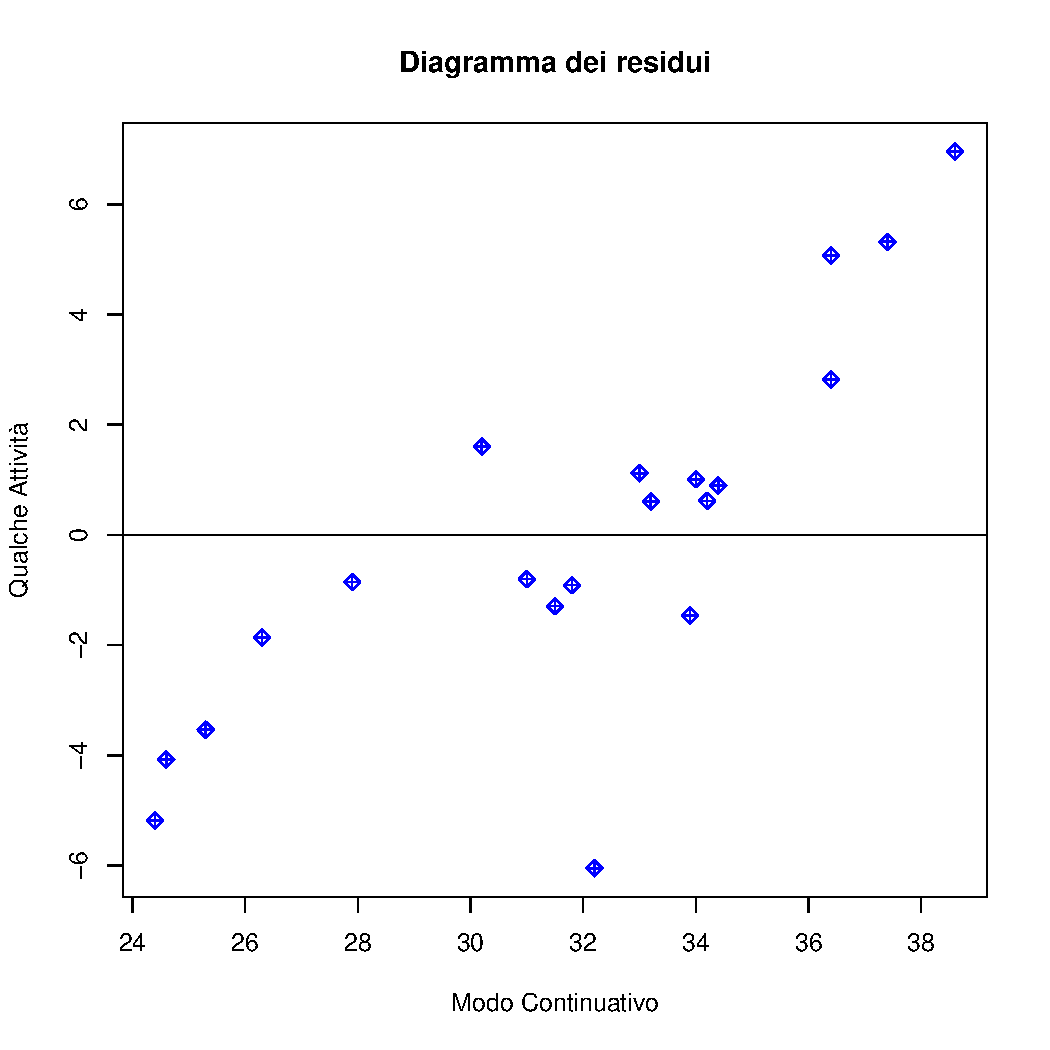
\includegraphics[height=16cm]{ProgettoSAD/capitoli/images/s_desc_biv/diagramma_residui.pdf}
\end{figure}
\vspace{5mm}

Nel grafico sovrastante si nota come sono disposti i residui rispetto alla variabile indipendente. La retta orizzontale è posizionata nello zero e corrisponde alla media campionaria dei residui, che è nulla. Si nota, inoltre, che i punti sono disposti in maniera abbastanza vicini alla retta, tranne che per alcuni valori che si discostano maggiormente.

Il diagramma dei residui aiuta a comprendere quale è l'adattamento della retta di regressione rispetto ai dati, notando che la posizione di tale retta è fortemente influenzata dalla presenza di eventuali valori anomali. Infatti, tale analisi aiuta a individuare i punti anomali dovuti a errori di stima. Si nota anche che eliminando i valori anomali, la varianza campionaria dei residui diminuisce.

\vspace{5mm}
\noindent \textbf{Residui standardizzati}
\vspace{5mm}

I residui standardizzati

\[E_i^{(s)} = \frac{E_i - \bar{E}}{s_E} = \frac{E_i}{s_E}\]

Risultano essere caratterizzati da media campionaria nulla e varianza unitaria. Di seguito, il codice per costruire il diagramma dei residui standardizzati con il relativo grafico:

\vspace{5mm}
\begin{lstlisting}
  standard_residue <- residuiValori(df) / sd(residuiValori(df))
  plot(stimeValori(df), standard_residue, main = " Residui standard rispetto ai valori stimati "
    , xlab = " Valori stimati ", ylab = " Residui standard ", pch = 4, col = " blue ")
  abline(h = 0, col = " red ", lty = 2)
\end{lstlisting}
\vspace{5mm}

\vspace{5mm}
\begin{figure}[!htbp]
    \centering
    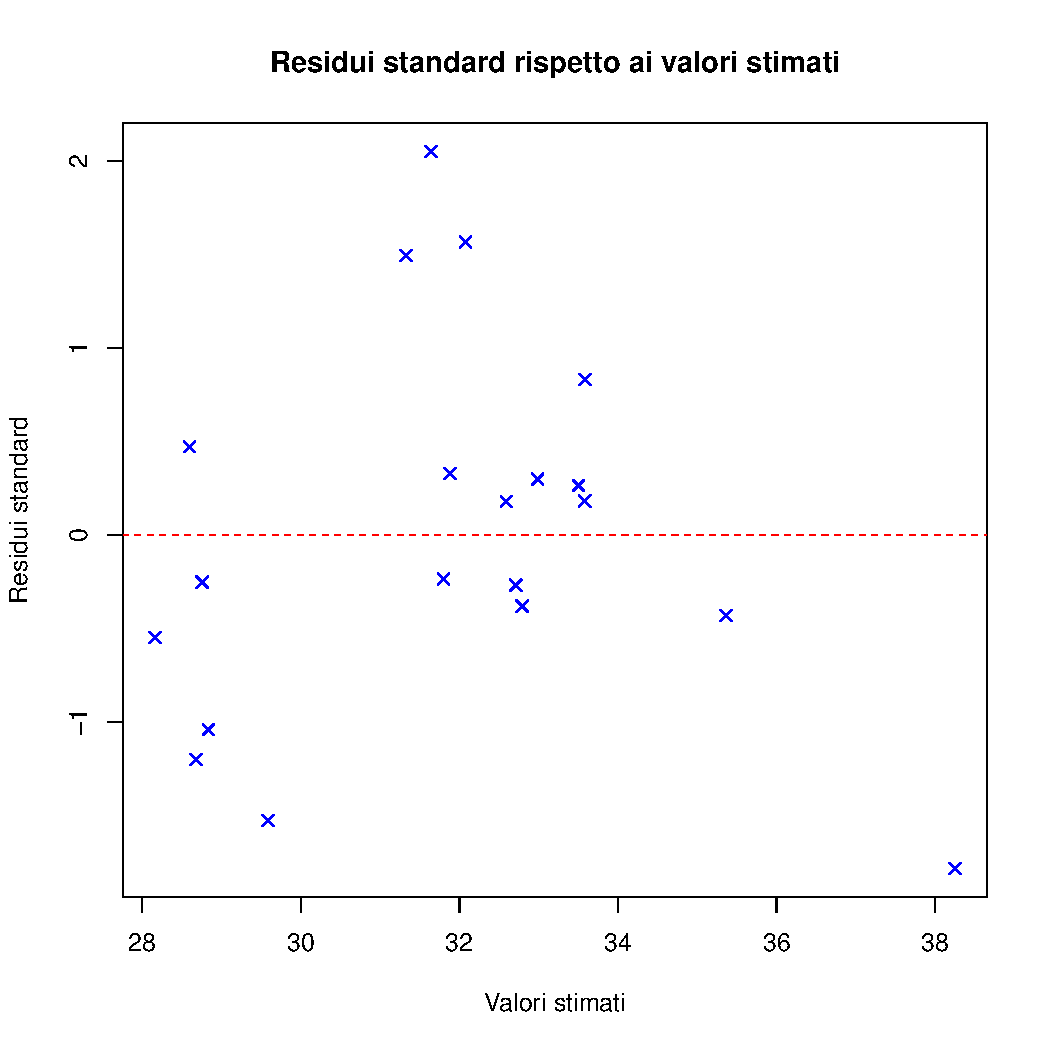
\includegraphics[height=16cm]{ProgettoSAD/capitoli/images/s_desc_biv/residui_standardizzati.pdf}
\end{figure}

Nel grafico sovrastante si nota come sono disposti i residui standardizzati rispetto ai valori stimati con la retta di regressione. La retta orizzontale è posizionata nello zero e corrisponde alla media campionaria dei residui standardizzati. Anche in questo caso i punti sono disposti in maniera abbastanza vicini alla retta, tranne per qualche che si discosta maggiormente.

\subsection{Coefficiente di determinazione}\label{cap4.2.2}

Poichè si è interessati a vedere quanto la retta si adatti ai dati, l'accento può essere posto sul quadrato del coefficiente di correlazione e su quanto esso si avvicini a uno.

\noindent \textbf{Definizione:} Se si denota con ($y_1, y_2, ..., y_n$) il vettore dei dati della variabile dipendente, con $\Bar{y}$ la sua media campionaria e con ($\hat{y_1}, \hat{y_2}, ..., \hat{y_n}$) i valori stimati attraverso la retta di regressione, il \textbf{coefficiente di determinazione} (r-square) è così definito:

\[D^2 = \frac{\frac{1}{n-1} \sum_{i=1}^n (\hat{y_i} - \Bar{y})^2}{\frac{1}{n-1} \sum_{i=1}^n (y_i - \Bar{y})^2} = \frac{\sum_{i=1}^n (\hat{y_i} - \Bar{y})^2}{\sum_{i=1}^n (y_i - \Bar{y})^2}\] 

Si noti che il coefficiente di determinazione è il rapporto tra la varianza dei valori stimati tramite la retta di regressione e la varianza dei valori osservati. Nel caso di regressione lineare semplice, il coefficiente di determinazione coincide con il quadrato del coefficiente di correlazione, ossia

\[D^2 = r_xy^2\]

In R si può calcolare il coefficiente di determinazione in due modi:

\vspace{5mm}
\begin{lstlisting}
(cor(df$Modo.Cont., df$Qualche.Att.))^2
[1] 0.3615508
summary (rettaRegressione(df))$r.square
[1] 0.3615508
\end{lstlisting}
\vspace{5mm}

Ottenendo un coefficiente di determinazione pari a 0.36 si potrebbe pensare che la retta di regressione non approssimi in maniera ottima i dati.

\section{Regressione lineare multipla}\label{cap4.3}

In molte applicazioni dell'analisi di regressione sono coinvolte situazioni con più di una singola variabile indipendente. Il modello di regressione lineare multipla viene utilizzato per spiegare la relazione tra una variabile quantitativa \textit{Y}, detta variabile \textit{dipendente}, e le variabili quantitative \textit{indipendenti} $X_1, X_2, ..., X_p$.

Il modello di \textbf{\textit{regressione lineare multipla}} con \textit{p} variabili indipendenti è esprimibile attraverso l'equazione:

\[Y = \alpha + \beta_1 X_1 + \beta_2 X_2 + ... + \beta_p X_p\]

dove 

\begin{itemize}
    \item $\alpha$ è l'intercetta, ovvero il valore di \textit{Y} quando $X_1 = X_2 = ... = X_p = 0$.
    \item $\beta_1, \beta_2, ..., \beta_p$ sono i regressori, dove $\beta_p$ rappresenta l'inclinazione di \textit{Y} rispetto alla variabile $X_p$ tenendo costanti le variabili $X_1, X_2, ..., X_{p-1}$.
\end{itemize}

Per lo studio della regressione lineare multipla si considera la caratteristica \textbf{Qualche Attività} come \textbf{variabile dipendente}, mentre le restanti variabili vengono considerate indipendenti.

\noindent \textbf{Scatterplot delle variabili}

\vspace{5mm}
\begin{lstlisting}
pairs(df, main = "Scatterplot per le coppie di variabili", col = "blue")
\end{lstlisting}
\vspace{5mm}

\vspace{5mm}
\begin{figure}[!htbp]
    \centering
    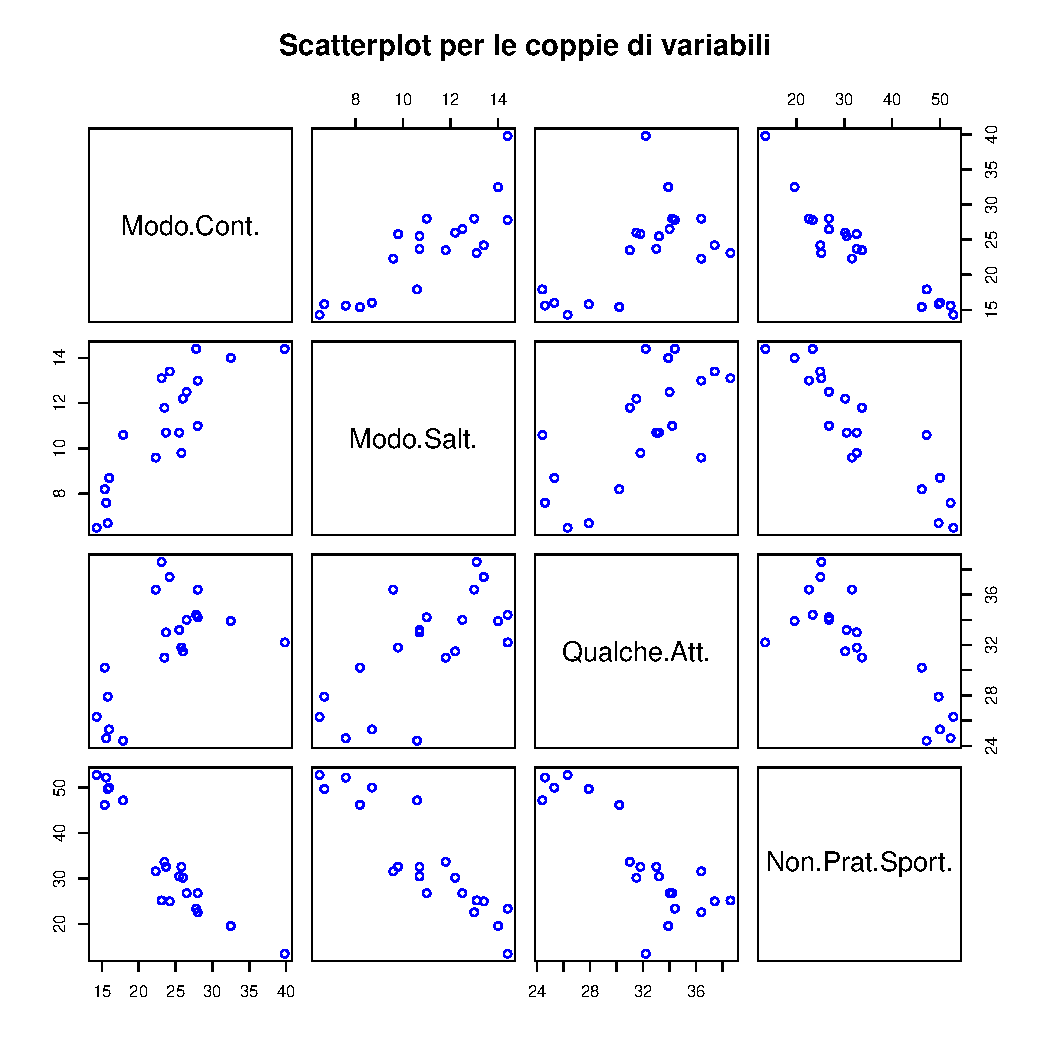
\includegraphics[height=16cm]{ProgettoSAD/capitoli/images/s_desc_biv/scatterplot_coppievariabili.pdf}
\end{figure}
\vspace{5mm}

La funzione \textit{pairs()} è in grado di visualizzare in un'unica finestra grafica una pluralità di scatterplot ottenuti mettendo in relazione tutte le coppie di variabili quantitative definite all'interno di un dataframe.

\noindent \textbf{Calcolo della retta di regressione}

Con il seguente codice si vanno a calcolare i valori dell'intercetta e dei regressori della retta:

\vspace{5mm}
\begin{lstlisting}
  lm_multiple <- lm(df$Qualche.Att. ~
                      df$Modo.Cont +
                        df$Modo.Salt. +
                        df$Non.Prat.Sport.)
  lm_multiple


Call:
lm(formula = df$Qualche.Att. ~ df$Modo.Cont + df$Modo.Salt. + 
    df$Non.Prat.Sport.)

Coefficients:
       (Intercept)        df$Modo.Cont       df$Modo.Salt.  df$Non.Prat.Sport.  
           99.6572             -1.0016             -0.9817             -0.9954  
\end{lstlisting}
\vspace{5mm}

In questo modo, si ottiene che l'intercetta è $\alpha = 99.65$, mentre i regressori sono $\beta_1 = -1.0016, \beta_2 = -0.9817, \beta_3 = -0.9954$.
Si può ora costruire la retta, ottenendo:

\[Y = 99.65 - 1.0016x_1 - 0.981x_2 - 0.995x_3\]

\subsection{Residui}\label{cap4.3.1}

Una volta calcolati i valori dei coefficienti $\alpha$, $\beta_1$, $\beta_2$, ..., $\beta_p$ è possibile osservare gli scostamenti (residui) tra le ordinate dei punti $y_i$ (valori osservati) e i corrispondenti valori stimati

\[\hat{y_i} = \alpha + \beta_1 x_{i, 1} + \beta_2 x_{i, 2} + ... + \beta_p x_{i, p} \quad (i = 1, 2, ..., n)\]

ottenuti mediante la regressione lineare multipla. I residui per la regressione multipla

\[E_i = y_i - \hat{y_i} = y_i - (\alpha + \beta_1 x_{i, 1} + \beta_2 x_{i, 2} + ... + \beta_p x_{i, p}) \quad (i = 1, 2, ..., n) \]

mostrano di quanto si discostano i valori osservati dai valori stimati con la retta di regressione. Anche in questo caso, la media campionaria dei residui $\Bar{E}$ è nulla, ossia in media gli scostamenti positivi e negativi si compensano.


\vspace{5mm}
\begin{lstlisting}
  residmulti <- resid(lm_multiple)
  residmulti

           1            2            3            4            5            6 
-0.078197132  0.048600345  0.023909012  0.045688728 -0.018641018  0.016097106 
           7            8            9           10           11           12 
 0.021131470  0.062707286 -0.167089936  0.034344833 -0.053011781  0.054154941 
          13           14           15           16           17           18 
 0.008837465  0.003505733 -0.097860973  0.059077439 -0.022290999  0.115289289 
          19           20 
-0.013064227 -0.043187582  
  
\end{lstlisting}
\vspace{5mm}

\noindent \textbf{Valori stimati}

\vspace{5mm}
\begin{lstlisting}
  stimemulti <- fitted(lm_multiple)
  stimemulti

       1        2        3        4        5        6        7        8 
31.57820 33.85140 38.57609 36.35431 32.21864 34.38390 37.37887 34.13729 
       9       10       11       12       13       14       15       16 
34.16709 32.96566 33.25301 31.74585 30.99116 30.19649 26.39786 24.34092 
      17       18       19       20 
25.32229 27.78471 24.61306 36.44319  
  
\end{lstlisting}
\vspace{5mm}

\noindent \textbf{Residui standardizzati}

Anche nel caso multivariato è interessante calcolare i residui standardizzati. Sono caratterizzati dalla media campionaria nulla e varianza unitaria. Di seguito il codice per costruire il diagramma dei residui standardizzati con il relativo grafico: 

\vspace{5mm}
\begin{lstlisting}
  standard_multi_resid <- residmulti / sd(residmulti)
  plot(stimemulti, standard_multi_resid
    , main =
         " Residui standard rispetto ai valori stimati "
    , xlab = " Valori stimati "
    , ylab = " Residui standard ", pch = 4, col = "blue")
  abline(h = 0, col = " red ", lty = 2)
\end{lstlisting}
\vspace{5mm}

\vspace{5mm}
\begin{figure}[!htbp]
    \centering
    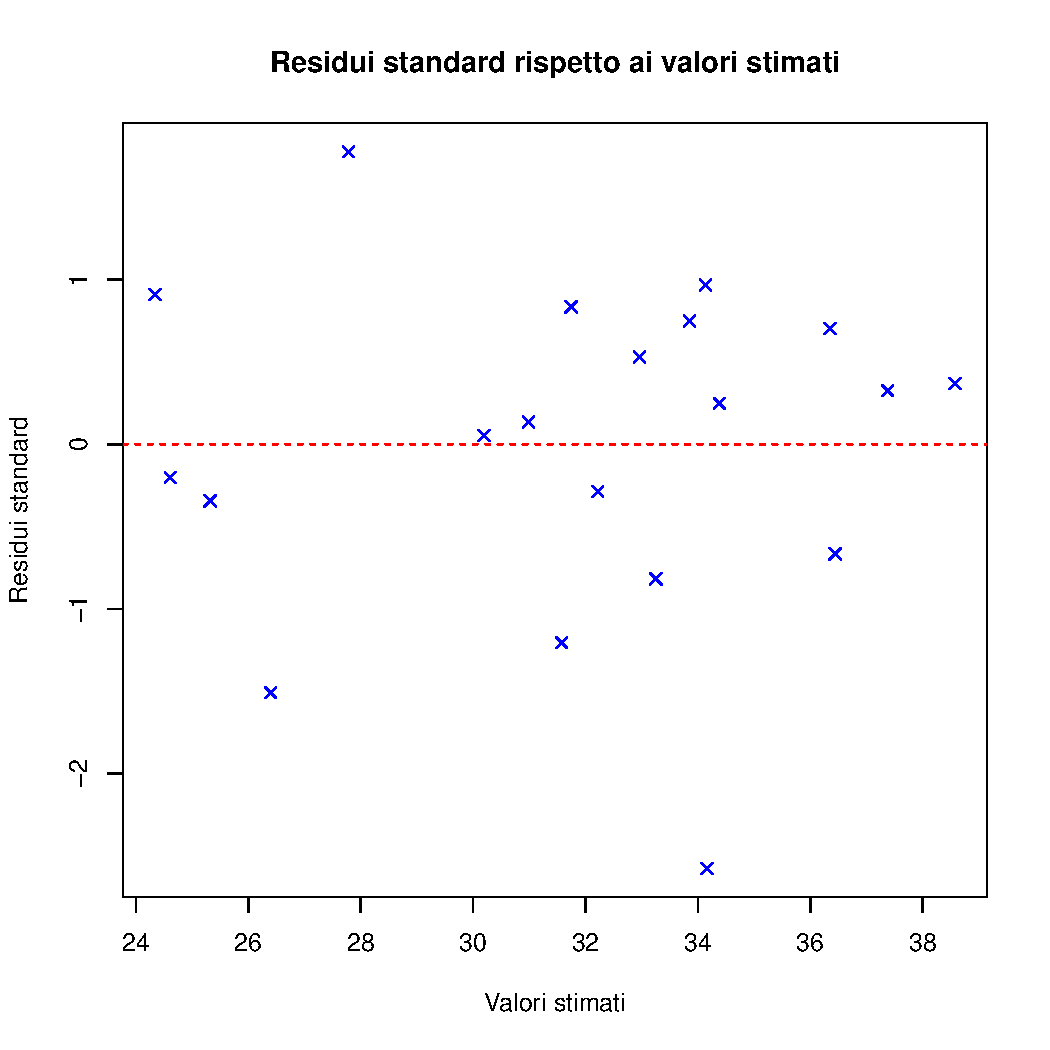
\includegraphics[height=16cm]{ProgettoSAD/capitoli/images/s_desc_biv/residui_standard_multipli.pdf}
\end{figure}
\vspace{5mm}

In questo caso i punti sono disposti quasi casualmente attorno alla retta e non si evidenzia nessuna tendenza particolare nella distribuzione dei punti.

\subsection{Coefficiente di determinazione}\label{cap4.3.2}

Il coefficiente di determinazione di un modello di regressione lineare multipla è il rapporto tra la varianza dei valori stimati tramite la funzione di regressione e la varianza dei valori osservati della variabile dipendente. Se si denota con ($y_1, y_2, ..., y_n$) il vettore dei dati della variabile dipendente, con $\Bar{y}$ la sua media campionaria e con ($\hat{y_1}, \hat{y_2}, ..., \hat{y_n}$) i valori stimati attraverso la funzione di regressione, il coefficiente di determinazione è:

\[D^2 = \frac{\frac{1}{n-1} \sum_{i=1}^n (\hat{y_i} - \Bar{y})^2}{\frac{1}{n-1} \sum_{i=1}^n (y_i - \Bar{y})^2} = \frac{\sum_{i=1}^n (\hat{y_i} - \Bar{y})^2}{\sum_{i=1}^n (y_i - \Bar{y})^2}\] 

L'indice $D^2$ è adimensionale e risulta $0 \leq  D^2 \leq 1$. Quando $D^2 = 0$ il modello di regressione multipla utilizzato non spiega per nulla i dati. Invece, quando $D^2 = 1$ il modello di regressione multipla utilizzato spiega perfettamente i dati.

In R si può calcolare il coefficiente di determinazione in due modi:

\vspace{5mm}
\begin{lstlisting}
  num <- sum((stimeMultipli(df) - mean(
    df$Modo.Salt.))^2)
  den <- sum((df$Modo.Salt. - mean(
    df$Modo.Salt.))^2)
  d2 <- num / den
  d2
  [1] 0.9997668

  summary(rettaRegressioneMultipla(df))$r.square
  [1] 0.9997668
\end{lstlisting}
\vspace{5mm}

Ottenendo un coefficiente di determinazione pari a 0.999 si può affermare che il modello di regressione multipla utilizzato può spiegare in maniera ottimale i dati.

\section{Regressione non lineare}\label{cap4.4}

In alcuni casi la regressione lineare non approssima bene i dati. Per tale motivo, si possono sfruttare modelli non lineari al fine di approssimare, nel miglior modo possibile, i dati a disposizione.

In particolare, in questo paragrafo si andrà ad analizzare la \textit{regressione polinomiale del secondo ordine}, considerando:

\begin{itemize}
    \item \textbf{Variabile indipendente: Modo Continuativo}
    \item \textbf{Variabile dipendente: Qualche Attività}
\end{itemize}

\subsection{Regressione polinomiale del secondo ordine}\label{cap4.4.1}

Consideriamo il modello non lineare

\[Y = \alpha + \beta X + \gamma X^2\]

dove Y è la variabile dipendente e X è la variabile indipendente.

\vspace{5mm}
\noindent \textbf{Scatterplot}

Con il seguente codice si vanno a visualizzare i punti delle due variabili all'interno di uno scatterplot: 

\vspace{5mm}
\begin{lstlisting}
  plot(df$Modo.Cont., df$Qualche.Att., main = " Scatterplot "
    , col = " blue ", xlab = " Modo Continuativo ",
       ylab = " Qualche Attività ")
\end{lstlisting}

\vspace{5mm}
\begin{figure}[!htbp]
    \centering
    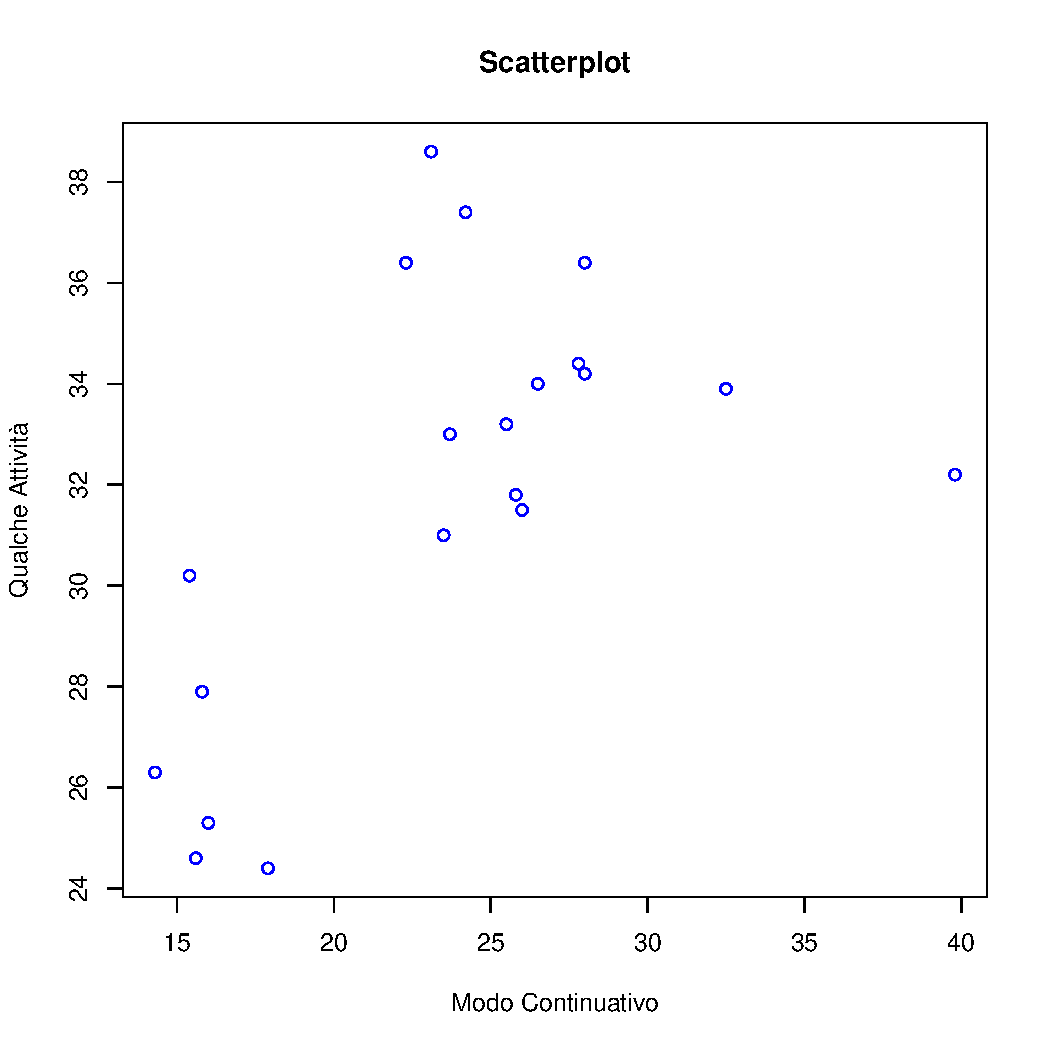
\includegraphics[height=16cm]{ProgettoSAD/capitoli/images/s_desc_biv/scatterplot_nonlineare.pdf}
\end{figure}
\vspace{5mm}

Vediamo se l'approssimazione con la regressione polinomiale del secondo ordine è adeguata per stimare i nostri dati. Le seguenti linee di codice:

\vspace{5mm}
\begin{lstlisting}
  lp <- lm(df$Qualche.Att. ~ df$Modo.Cont. + I(df$Modo.Cont.^2))
  lp

  Coefficients:
       (Intercept)       df$Modo.Cont.  I(df$Modo.Cont.^2)  
           0.49050             2.27820            -0.03757
\end{lstlisting}
\vspace{5mm}

mostrano che $\alpha = 0.4905, \beta = 2.27820$ e $\gamma = -0.03757$, ottenendo:

\[Y = 0.4905 - 2.27820*X + -0.03757*X^2 \]

\noindent \textbf{Disegno Curva}

Disegnando la curva sul grafico si ottiene:

\vspace{5mm}
\begin{lstlisting}
  alpha <- 0.4905
  beta <- 2.27820
  gamma <- -0.03757
  plot(df$Modo.Cont., df$Qualche.Att., main = " Scatterplot e curva stimata "
    , col = " blue ", xlab = " Modo Continuativo ",
       ylab = " Qualche Attività ")
  curve(alpha + beta * x + gamma * x^2, add = TRUE)
\end{lstlisting}
\vspace{5mm}


\vspace{5mm}
\begin{figure}[!htbp]
    \centering
    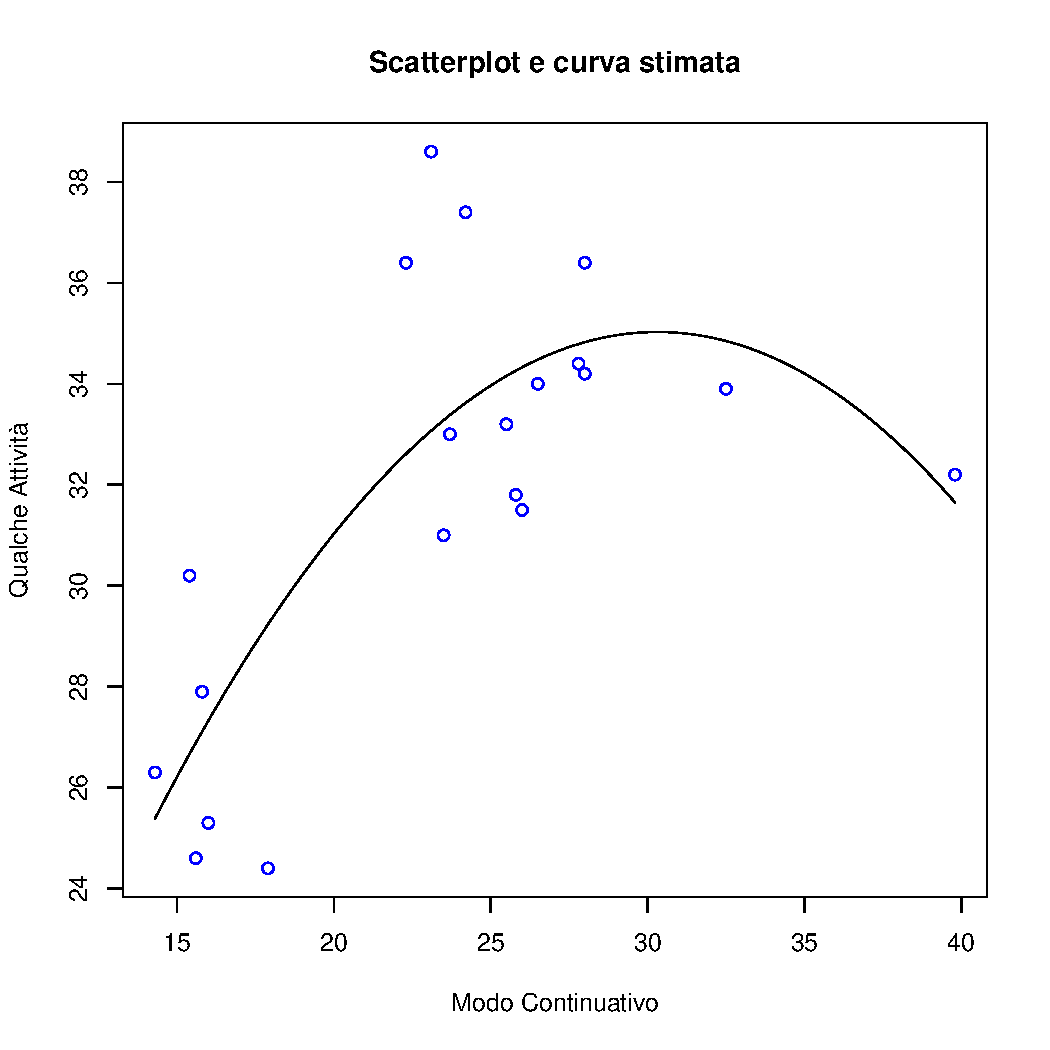
\includegraphics[height=16cm]{ProgettoSAD/capitoli/images/s_desc_biv/scatterplot_nonlin_curva.pdf}
\end{figure}
\vspace{5mm}

\noindent \textbf{Residui}

Calcolando anche i residui il grafico viene così aggiornato:

\vspace{5mm}
\begin{lstlisting}
#Questo codice viene aggiunto al precedente per creare il plot

  segments(df$Modo.Cont., stime, df$Modo.Cont.
    , df$Qualche.Att., col = " green ")
\end{lstlisting}
\vspace{5mm}

\vspace{5mm}
\begin{figure}[!htbp]
    \centering
    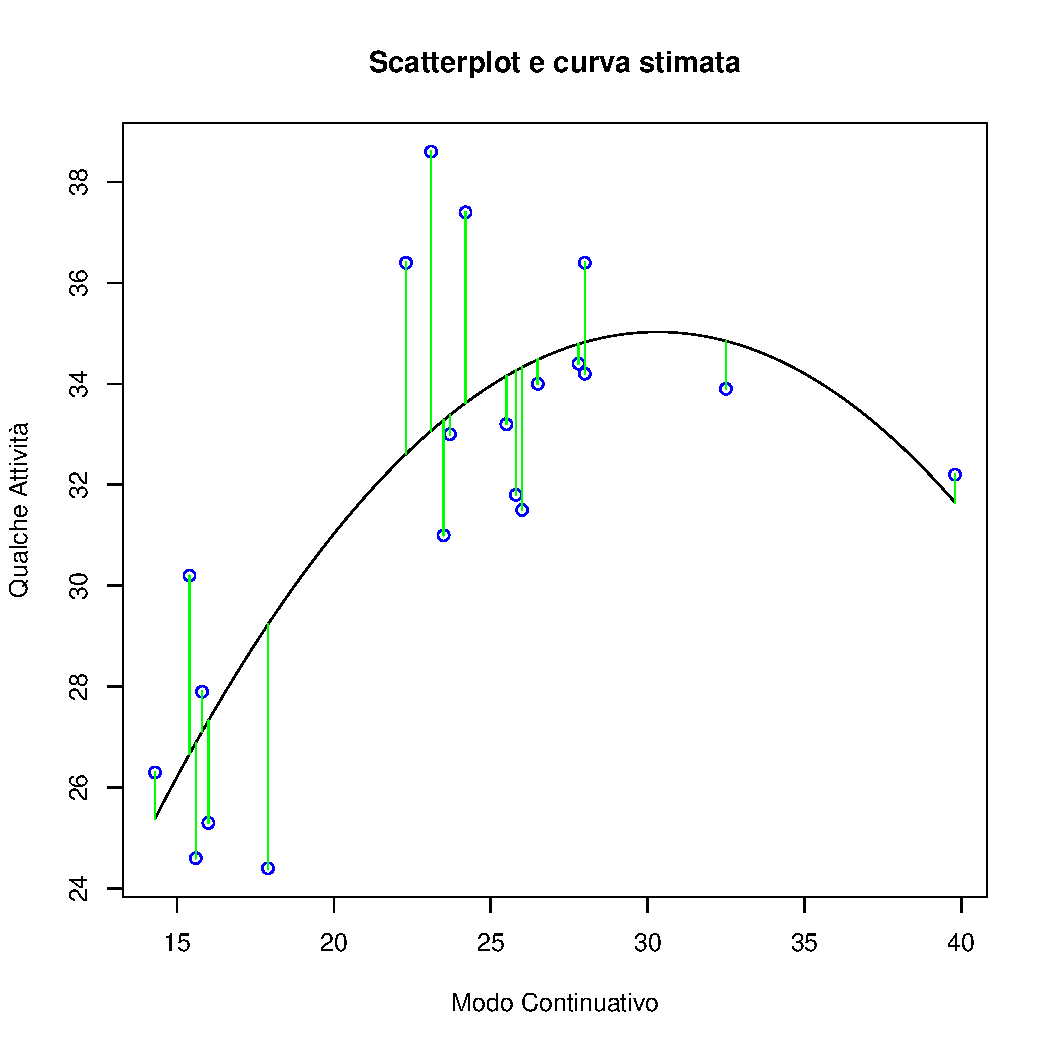
\includegraphics[height=16cm]{ProgettoSAD/capitoli/images/s_desc_biv/scatter_nonlin_resid.pdf}
\end{figure}
\vspace{5mm}

\noindent \textbf{Coefficiente di Determinazione}

Il calcolo del coefficiente di determinazione:

\vspace{5mm}
\begin{lstlisting}
    summary ( rettaRegressioneNonLin(df) )$r.square
  [1] 0.6189822
\end{lstlisting}
\vspace{5mm}

Si può osservare che, con la regressione non lineare, si ottiene un risultato migliore rispetto a quello ottenuto con la regressione lineare.


%################################################

\newpage